\section{Applications}\label{sec::applications}
\subsection{Introduction}
The last chapters described in detail the different components involved in our Visual Analytics approach for comparing tree-structures. This chapter exemplary studies three usage scenarios and describes additional preprocessing steps if necessary. To demonstrate the feasability of our approach with real world data the following three applications are studied:

\begin{itemize}
\item Import of Lexical Functional Grammar (LFG) XML exported files.
\item Import of sorted Wikipedia articles by revision-timestamps. 
\item A Directory recursively watched for changes within a filesystem. The XML representation thereof is based on FSML\cite{FSML}. 
\end{itemize}

\subsection{LFG}
Linguists often face the problem of having to compare Abstract Syntax Trees (ASTs). The LFG (Lexical functional grammar) in particular differenciates between two structures:

\begin{enumerate}
\item{Constituent structures (c-structures)} which "have the form of context-free phrase structure trees".
\item{Functional structures (f-structures)} "are sets of pairs of attributes and values; attributes may be features, such as tense and gender, or functions, such as subject and object."\cite{LFG}
\end{enumerate}

We obtained an XML-export of a collection of different versions of a c-structure/f-structure combination. To import differences between these XML documents in Treetank the FMSE-algorithm described in Chapter \ref{sec::relwork} and \ref{sec::differences} is used for the simple reason that the XML-export does not include unique node identifiers. Thus we can not rely on node-IDs and have to figure out differences using our similarity metrics defined for leaf- and inner-nodes. Fig. \ref{fig:lfg} illustrates the visualization of a diff between two revisions.

\begin{figure}[tb]
\center{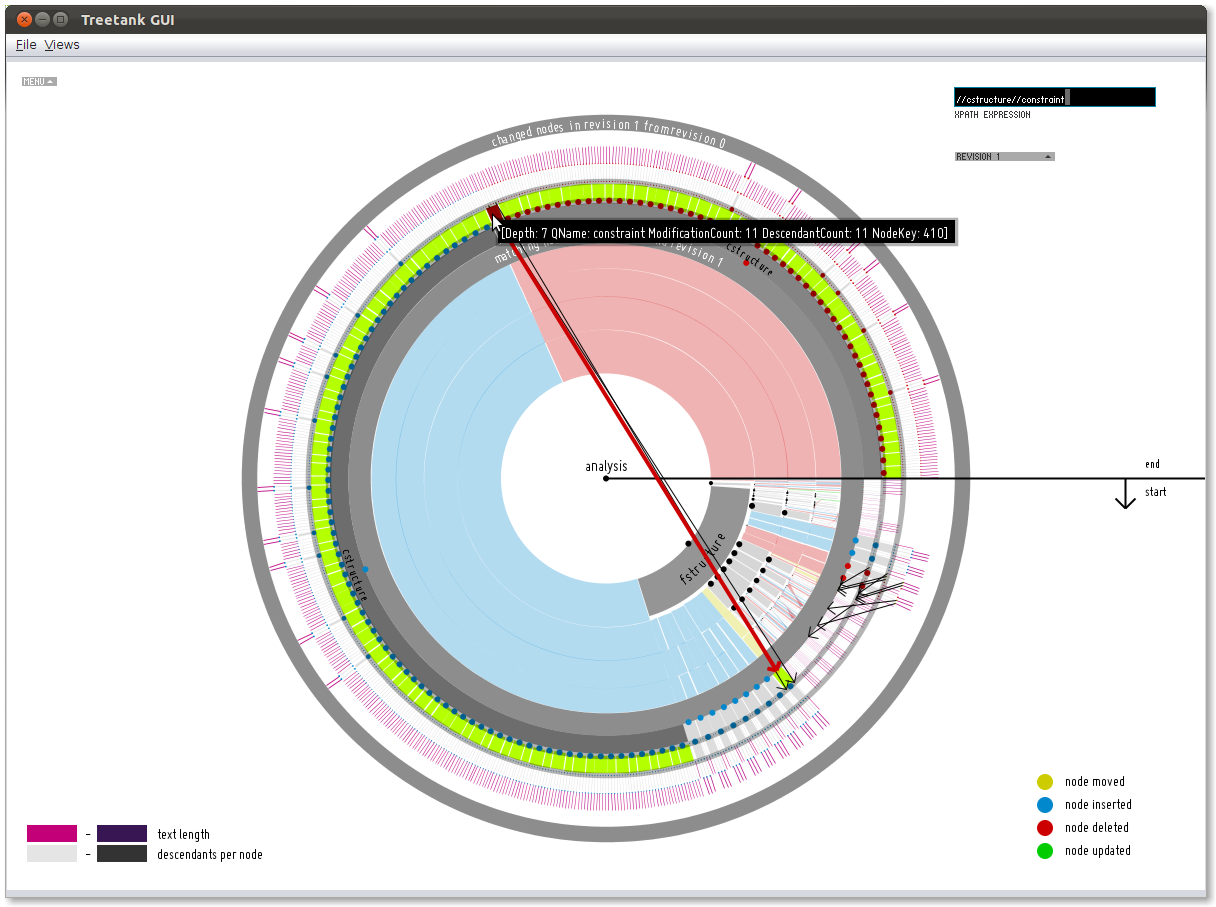
\includegraphics[width=\textwidth]
{figures/lfg.png}}
\caption{\label{fig:lfg} LFG comparsion}
\end{figure}

It is immediately obvious by investigating the original XML-documents, that the FMSE-algorithm mismatched nodes in the first place which in effect causes a lot of edit-operations. Nodes are touched which are not changed and vice versa\footnote{note, that the final outcome is nontheless correct in terms of the first tree-structure is correctly edited to represent the second}. Thus, the FMSE-algorithm does not generate a minimum edit-script and executes too many edit-operations especially in case of the deletion and reinsertion of the old- respectively the new-\texttt{cstructure} subtree. In doing so, a subsequent visualization is impractical, for the simple reason that it almost mirrors the update-operations issued by the FMSE-algorithm for consecutive versions. As stated in Chapter \ref{sec::relwork} ID-less algorithms work best if leaf nodes and therefore especially text-nodes are very well distinguishable. That is the initial matching of leaf nodes in most if not all cases really matches unchanged nodes, which is the desired behavior. 

Having a close look at the input documents reveals a lot of changed or updated text-values (Listing \ref{lst:linguistscomparsion}). Our threshold value for matching subtrees in case of inner nodes is $0.5$ (has to be $> 0.5$ for matching nodes) and thus the arg-elements are not matched.

For that reason we changed the leaf-node comparison slightly. Instead of just relying on the Levenshtein-distance for text-node values we also try to match all ancestor \texttt{QName}s \footnote{ancestors are always element nodes, the document-root node is not visited} if the returned normalized value is $<=$ the threshold value defined for the similarity of leaf nodes. Note that only leaf nodes are considered to match if the threshold is $>$ than the predefined threshold. Hence, the leaf nodes are matched and "updated" by FMSE instead of deleting/inserting the whole subtree.

The result is depicted in Fig. \ref{fig:linguistics}.

\begin{figure}[tb]
\center{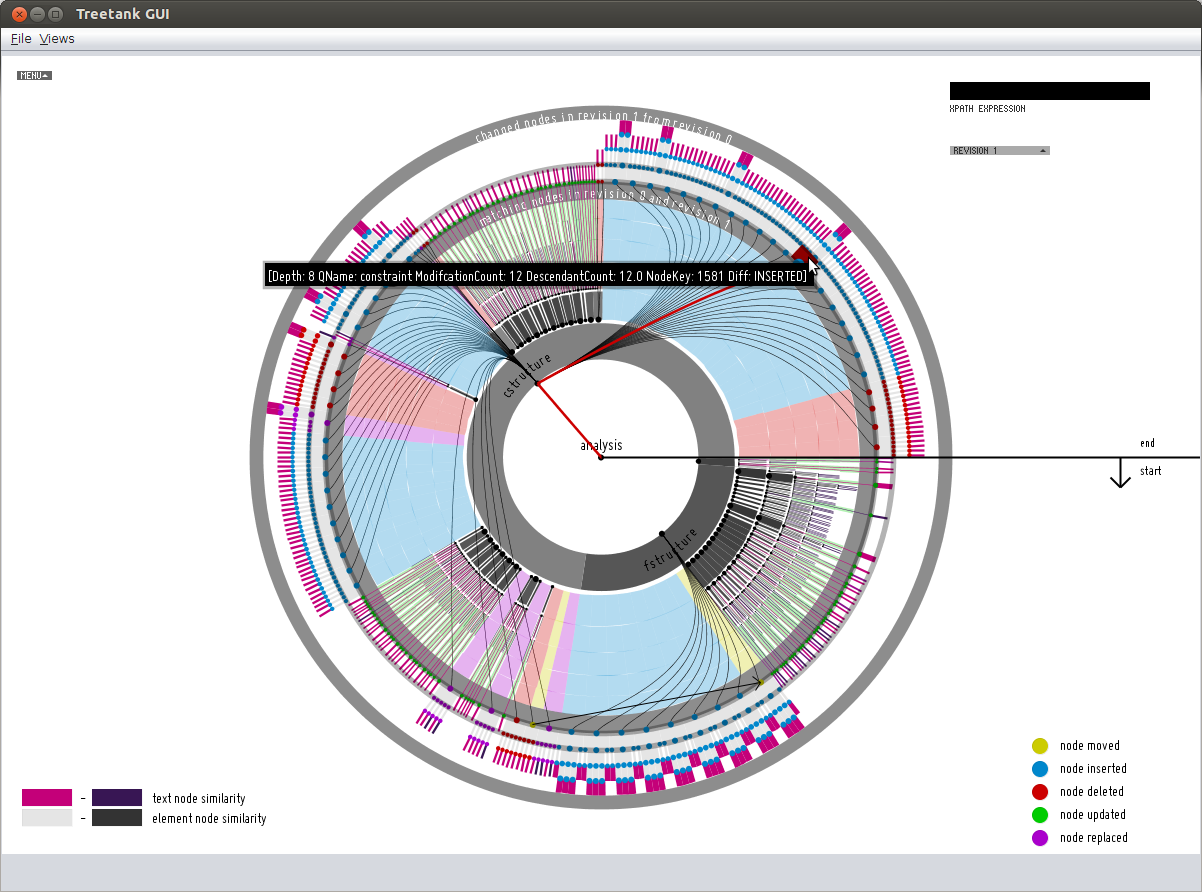
\includegraphics[width=\textwidth]
{figures/linguistics.png}}
\caption{\label{fig:linguistics} LFG comparsion revised}
\end{figure}

We observe that still many nodes are changed, but by looking at the original XML-documents we observe that indeed a lot of nodes have been updated/deleted/inserted or replaced. For instance by scrolling both XML-documents at the end of the fstructure-subtree a lot of subtrees must have been inserted.

\begin{code}[caption=CStructure/FStructure comparsion]
<cstructure>                   <cstructure>
  <constraint>                   <constraint>
    <label>subtree</label>         <label>subtree</label>
    <arg no="1">102</arg>          <arg no="1">163</arg>
    <arg no="2">ROOT</arg>         <arg no="2">ROOT</arg>   
    <arg no="3">-</arg>            <arg no="3">-</arg>
    <arg no="4">83</arg>           <arg no="4">145</arg>
  </constraint>                  </constraint>
  <constraint>                   <constraint>
    <label>phi</label>             <label>phi</label>
    <arg no="1">102</arg>          <arg no="1">163</arg>
    <arg no="2">var:0</arg>        <arg no="2">var:0</arg>
  </constraint>                  </constraint>
  ...                            ...
</cstructure>                  </cstructure>
\end{code}
\label{lst:linguistscomparsion}

However as a direct consequence of this short evaluation it is inevitable to rely on unique node identifiers if we want to visualize minimal edit-scripts in case of updated leaf node values which are very distinct to the other trees' leaf node values or worse the leaf nodes are very similar. Comparisons based on similarity-metrics are always based on heuristics. Assuming the export of the XML-documents includes unique identifiers of the nodes, importing requires utilization of the internal diff-algorithm to simply store incremental changes, the changes from the old- to the new-revision. The following steps have to be implemented:

\begin{enumerate}
\item Import of the initial XML-document.
\item Import the first updated XML-document to a temporary resource.
\item Utilize the internal Treetank diff-algorithm to determine changes based on unique node-IDs. Whenever an edit-operation is encountered the appropriate transaction-method has to be executed. %In case of \texttt{element}- and \texttt{text}-nodes it requires how to insert nodes\footnote{remember that Treetank currently is able to insert a node as a right sibling or first child} and where, which is very simple due to the \texttt{transaction.moveTo(long)}-method which can move the transaction/cursor directly to the left-sibling-node of the node to insert if it is available or to the parent. In the first case the node has to be inserted as a right sibling, in the latter case as a first child of the parent node.
\end{enumerate}

Furthermore this approach applies to every XML-document which incorporates unique node identifiers.

Next, we study the import of several articles from Wikipedia ordered by timestamp of their revisions. 

\subsection{Wikipedia}
Wikipedia is studied as an application to demonstrate the feasability of our approach on a large text corpora. However several issues have to be solved during preprocessing.

\begin{itemize}
\item Wikipedia is dumped as a very large XML-file. "'The XML itself contains complete, raw text of every revision"'\cite{WikiDump} and thus is a full dump instead of an incremental- or differential-dump describing the changes an author performed. Appendix \ref{sec::wikidump} depicts a small example of the structure of an Wikipedia XML-dump. Moreover WikiText, which is a proprietary markup format is stored as plain text and not replaced by XML-markup. Thus, the content of an article in each revision is a huge \texttt{TextNode} which includes the full text instead of just denoting the changes and its context in some form. Differences between the actual content of several revisions of an article on a node-granular level can not be found with a state of the art native XML database system, which supports revisioning of the data, as a direct consequence. The database systems' best bet is to generate a character based delta between the two large text-nodes.

\item Furthermore due to the fact that XPath 2.0 should be usable without requiring an XQuery/XPath Full Text 1.0 implementation and our overall goal is to analyse the temporal evolution of the stored data, WikiText markup has to be converted into semistructured XML fragments. To accomplish this the Wiki2XML parser from the MODIS team \cite{Wiki2XML} is used.

\item Another issue arises because the Wikipedia dump is not sorted and we want to analyse and visualize the temporal evolution during several snapshots. Neither articles are sorted by date/time nor revisions of the articles are. Thus for the subsequent revisioned import the revisions have to be sorted with their associated article metadata (page id, author...). For the simple reason that we have to deal with large amounts of data an external sorting algorithm has to be used. Instead of implementing an own approach, Hadoop is a natural choice. Its \emph{MapReduce}\cite{Hadoop} framework is a "programming model and software framework for writing applications that rapidly process vast amounts of data in parallel on large clusters of compute nodes". The overall process of the programming model is divided into two functions.
\end{itemize}

\begin{enumerate}
\item \texttt{Map} is a function that splits the problem into subproblems are distributed among worker nodes in a cluster. Logically it is a function of the form \texttt{$Map(k1,v1) \rightarrow list(k2,v2)$} where $k1$ and $v1$ is an input $key$ and $value$ and the output from the function is a list of $key/value$ pairs (\texttt{list(k2, v2)}). After that the MapReduce framework groups the values according to the keys.
\item \texttt{Reduce} is a function of the form: \texttt{$Reduce(k2, list (v2)) \rightarrow list(v3)$}. It receives a $key$ and a list of grouped $values$ and performs any computation which might be feasable and returns another list of $values$.
\end{enumerate}

The \texttt{map}-function receives input data splitted into records. Most MapReduce frameworks rely on a programmable mechanism to do this. In Hadoop it is the responsibility of the \texttt{InputStream} in conjunction with a \texttt{RecordReader}. The following steps describe the implementation of sorting Wikipedia by Hadoop.

\begin{enumerate}
\item \texttt{XMLInputStream} in conjunction with an \texttt{XMLRecordReader} splits records on \emph{revision-elements} with the \emph{page}-metadata prepended. The \textbf{timestamp} of each revision denotes the key, the whole subtree of each \emph{revision}-element is saved as the value for the \texttt{map} input. The algorithm is straight forward. A \texttt{SAX-Parser} is used to determine starting and ending of each record.

The implementation utilizes a configurable record identifier such that it is adjustable to schema changes in the Wikipedia dump. 

\item \texttt{XMLMap} just forwards the received key/value pairs.
\item \texttt{XMLReduce} finally merges consecutive revisions with the same \emph{page-id} and \textbf{timestamp} by means of Saxon, an XSLT/XQuery-processor. Our XSLT stylesheet to achieve the concatenation is small yet maybe not straight forward (Appendix \ref{sec::xslt}).
\end{enumerate}

% import of wikipedia
Once the dump is sorted with MapReduce it has to be imported into Treetank. First of all, as we have splitted the data on \texttt{revision}-elements and pre\-pen\-ded the \texttt{page-}metadata we have to construct a new root node, which is simply done by prepending a \texttt{mediawiki} start-tag, then writing the result of the Hadoop-run and appending a corresponding end-tag to a new file. Otherwise it is no valid XML-document and can not be parsed by XML-parsers.

Next, it is the responsibility of a Wikipedia-Importer to import the revisioned file which is now in ascending timestamp order of all revisions from all pages/articles. It utilizes the FSME-implementation described in detail in Chapter \ref{sec::relwork} and \ref{sec::differences} to just import incremental changes between the latest stored revision in Treetank and a shredded List of \texttt{XMLEvent}s in a temporary database/resource. Therefore as data is read-in from the XML document with a StAX-Parser the page-metadata as well as the whole revision-subtree is saved in a simple main-memory collection, a \texttt{List}, assuming the XML-content of an article can be put in main memory. The assumption holds true as every revision can be parsed and rendered in a web-browser. Everytime a \texttt{page} end-tag is encountered the page-id is searched in the already shreddered revision. If it is found the FMSE algorithm is called for the found \texttt{page}-element, such that the encountered differences are shreddered subsequently. In case the XPath expression returns no results, that is the page-ID is not found a new page is going to be appended as a right sibling to the last \texttt{page}-element.

The Importer for Wikipedia allows the usage of a timespan (hourly, daily, monthly, yearly) which is used for the revisioning. Whenever a new timestamp is encountered, which differs from the current timestamp depending on the chosen timespan the transaction is commited.

Fig. \ref{fig:wikivis} demonstrates the result of importing 50 articles of Wikipedia sorted by article-revisions and an hourly commit \footnote{only hours in which changes occured are reflected}. Revisions 70 and 71 are compared. The \emph{edit-distance} used by our FSME-implementation to determine and update the stored Treetank-data with the encountered differences in the first place works reasonably well, as most text-nodes are distinguishable very well. We used the hash-based pruning to enlarge regions of interest. The \emph{TextView} on the right side is particular useful to quickly reveal several changes in particular updated text whereas a label in the \emph{SunburstView} only depicts the new updated text content in case of \texttt{TextNode} updates and usually the content is too big to be displayed within the arc, especially if the content contains whole paragraphs as is usually the case for Wikipedia. Both text values, the old- and the new-value is displayed on mouseover. We quickly detect that a lot of paragraphs have changed by looking at the \emph{SunburstView}. Details are depicted by either hovering an item or scrolling down in the \emph{TextView}. %It is fair to say, that for instance the text-nodes below the \texttt{id}-element parent could be detected as updates as well if all ancestors and neighbour nodes are checked for equality even though the Levenshtein algorithm used to compare text nodes detects too many character edit operations to consider that the nodes are equal. 

\begin{figure}[tb]
\center{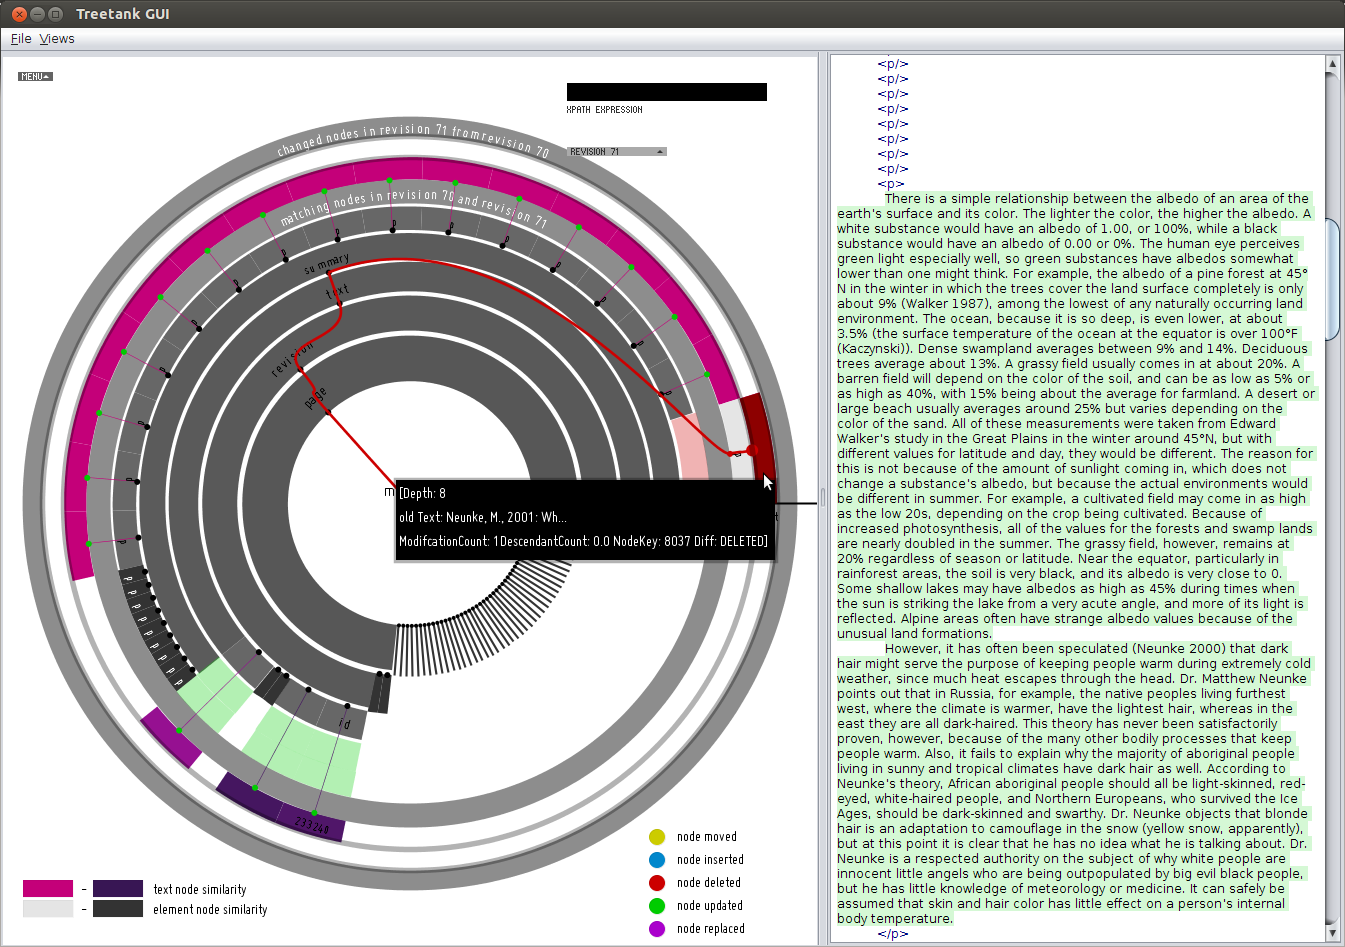
\includegraphics[width=\textwidth]
{figures/wikipedia-rev7071}}
\caption{\label{fig:wikivis} Wikipedia comparsion.}
\end{figure}

Another visualization (Fig. \ref{fig:wikivis-without-modscale}) depicts the situation without pruning and without including the number of modifications of a node in its subtree to scale the Sunburst items, the segments for each node.

\begin{figure}[tb]
\center{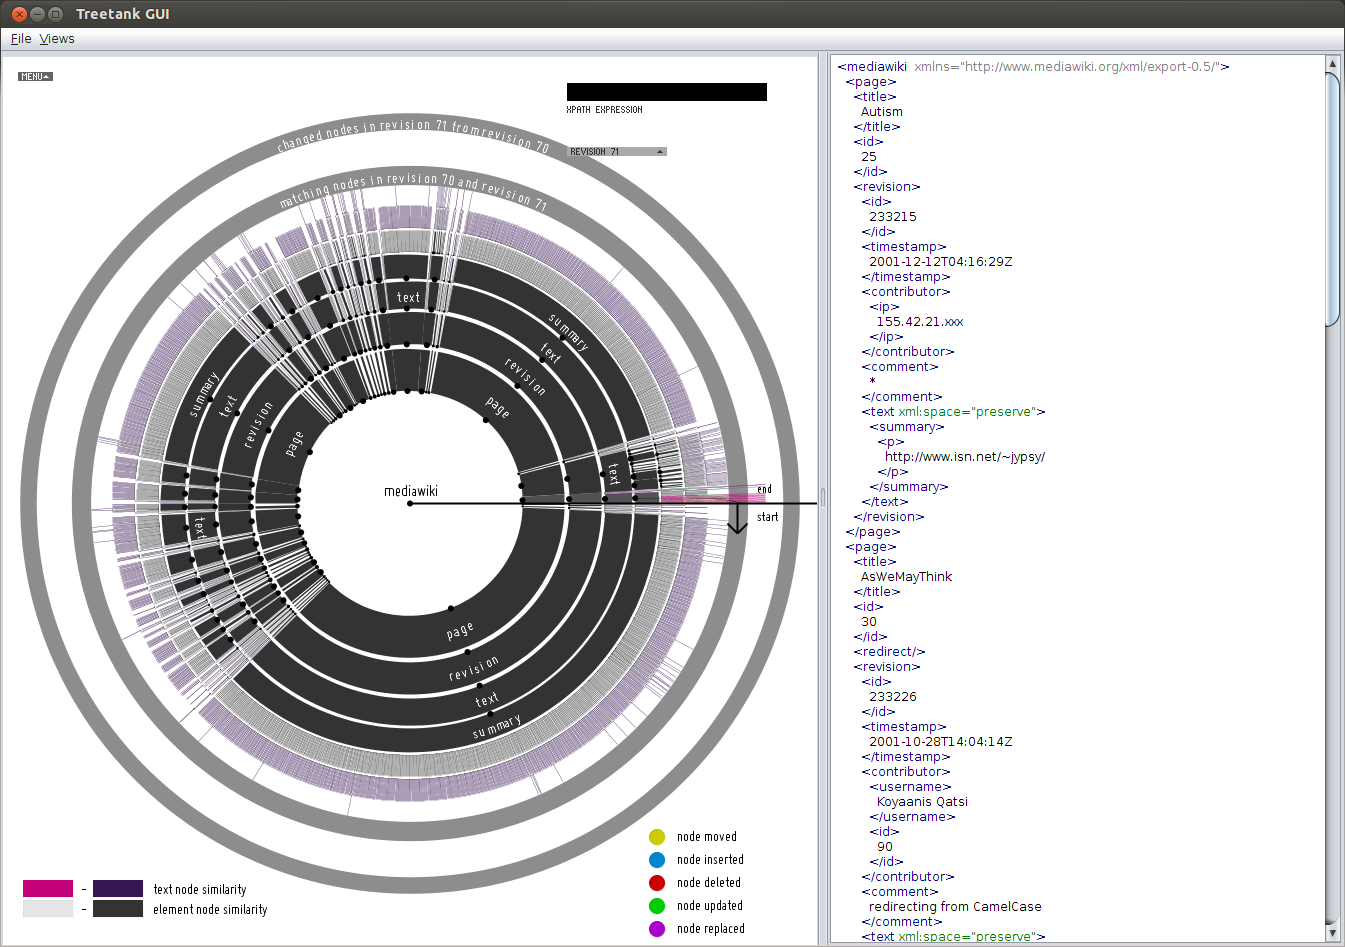
\includegraphics[width=\textwidth]
{figures/wikipedia-without-pruned-modifications}}
\caption{\label{fig:wikivis-without-modscale} Wikipedia comparsion without pruning and including the modification weight to determine the size of a SunburstItem}
\end{figure}

The changes in the last page/article are hardly visible. Most items denote unchanged nodes without any modifications in their subtree and thus do not carry any useful information, if we just want to quickly determine changes. This and the fact that we do not include the modification weight to scale items, that is only the subtree size of each node matters, results in considerably reduced itemsizes of changed items.

Despite viewing changes between subsequent revisions which in case of importing only 50 articles most often results in appending or updating one article it is possible to view changes between arbitrary revisions. Fig. \ref{fig:wikivis-rev90106} reveals changes between revision 90 and 106. Thus seven articles have changed and it is very easy to determine regions of interest and to further drill down into the tree through selecting a new root node in the \emph{SunburstView}. The page/article with the name "ArgumentForms" has been changed considerably. The page-nodes which are containers of the whole article do not have enough matching subtree-nodes in common between the two revisions, such that they are not matched, too. The FMSE-algorithm thus deletes the whole article and inserts the article as a new first child of the "wikimedia" root-element. The changes in the other articles mainly either include single paragraphs which are updated or larger subtrees which are replaced. Detailed changes are depicted on demand, that is if we drill down into the tree and/or scroll down in the \emph{TreeView}. The transparent red square in the \emph{SunburstView} in Fig. \ref{fig:wikivis-rev90106} illustrates the article/page to which we have scrolled in the \emph{TextView}.

\begin{figure}[htb]
\center{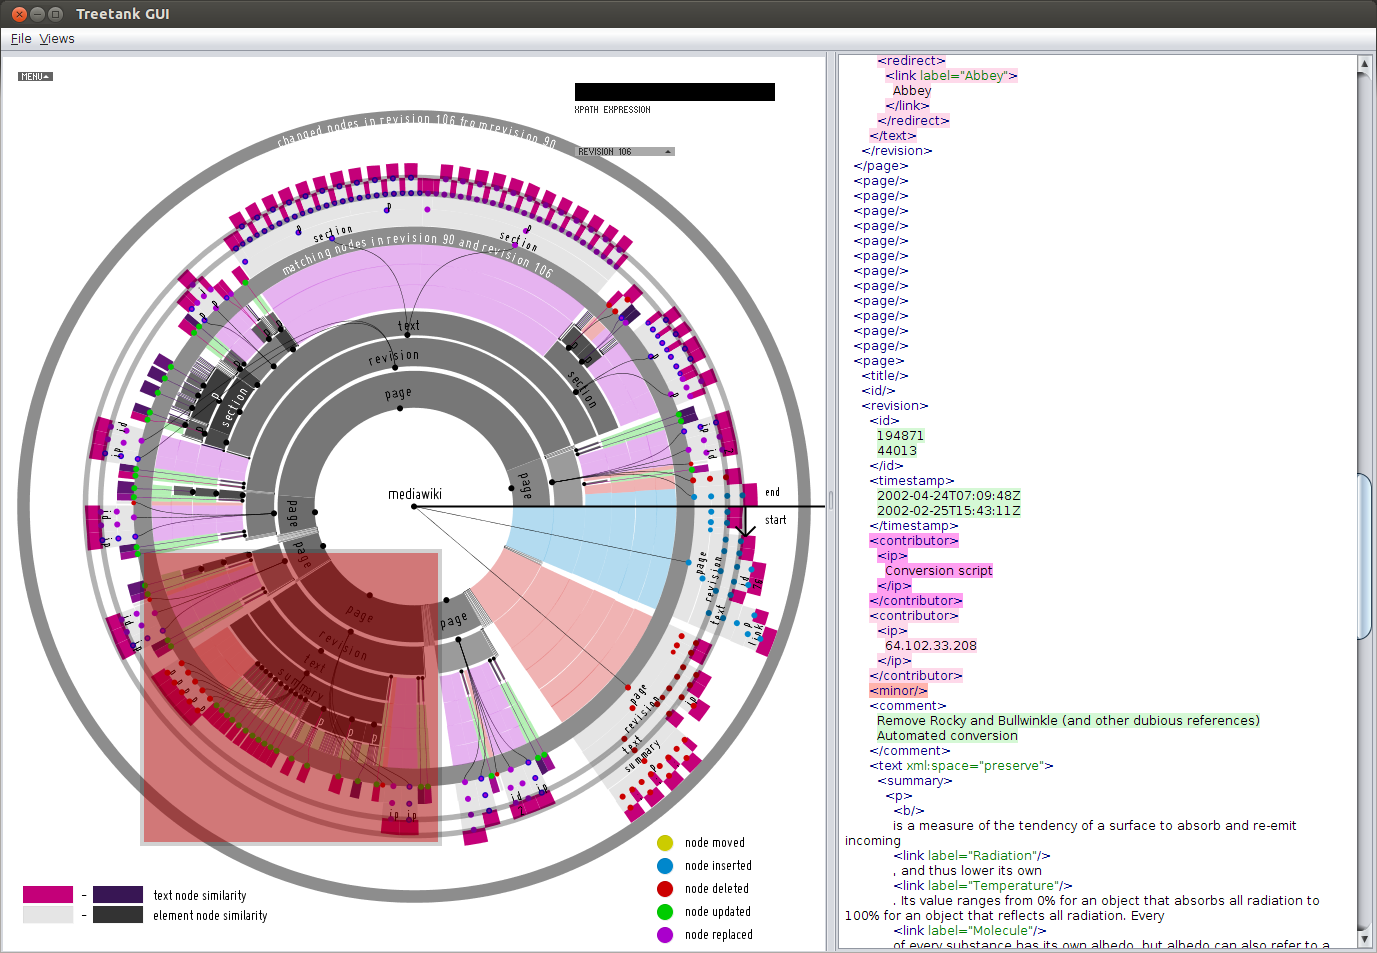
\includegraphics[width=\textwidth]
{figures/wikipedia-rev90106}}
\caption{\label{fig:wikivis-rev90106} Wikipedia comparsion pruned by itemsize}
\end{figure}

Besides comparing only two revisions small multiple display variants facilitate the comparison between several revisions (currently at most five revisions). Fig. \ref{fig:wikipedia-incremental} illustrates changes between revisions 70,71 (upper left), 71,72 (upper right), 72,73 (bottom right) and 73,74 (bottom left). We are quickly able to determine that except in the SunburstView comparing revisions 73 and 74 all other small multiples change or delete/insert the same article. The comparison between revision 70,71 and 72,73 reveal a lot of updated paragraphs. Between revisions 71 and 72 the same article has been deleted and inserted. We are quickly able to determine that a lot of paragraphs have been added as the inserted article includes more descendants than the article in the old revision. Thus the FMSE-algorithm does not match the page-nodes due to very different subtrees. Repacitulate that in order to match inner nodes, more than at least half of the nodes in both subtrees have to be matched. To gain a better understanding about the differences between revision 73 and 74 we switch to the \emph{SunburstView} in conjunction with the \emph{TextView}. We are able to quickly determine that the deleted and inserted page denotes the same article (autism) once more (Fig. \ref{fig:wikipedia-rev7374}). The article changed from a single paragraph which just included a URL to a slightly more profound description of autism.

\begin{figure}[tb]
\center{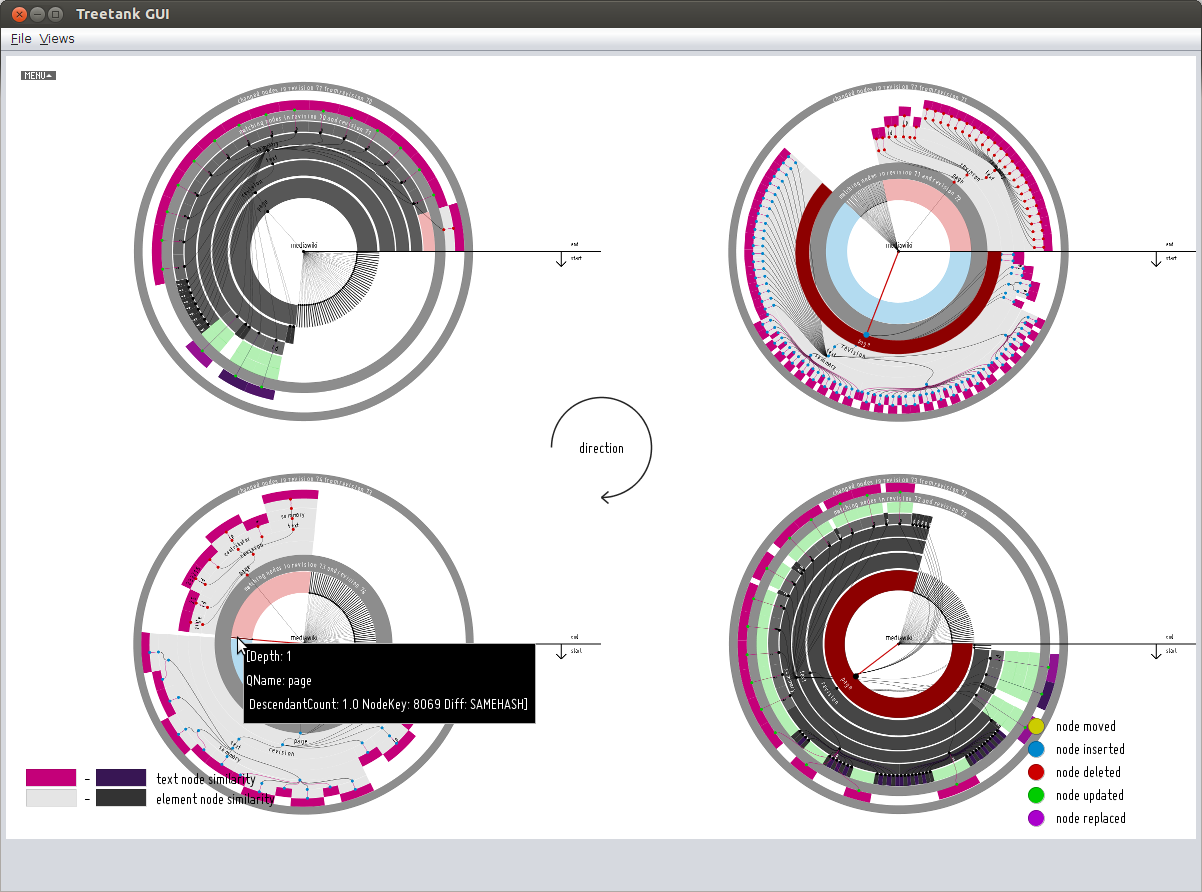
\includegraphics[width=\textwidth]
{figures/wikipedia-incremental}}
\caption{\label{fig:wikipedia-incremental} Wikipedia comparsion - depicting differences through the incremental smallmulltiple variant}
\end{figure}

\begin{figure}[tb]
\center{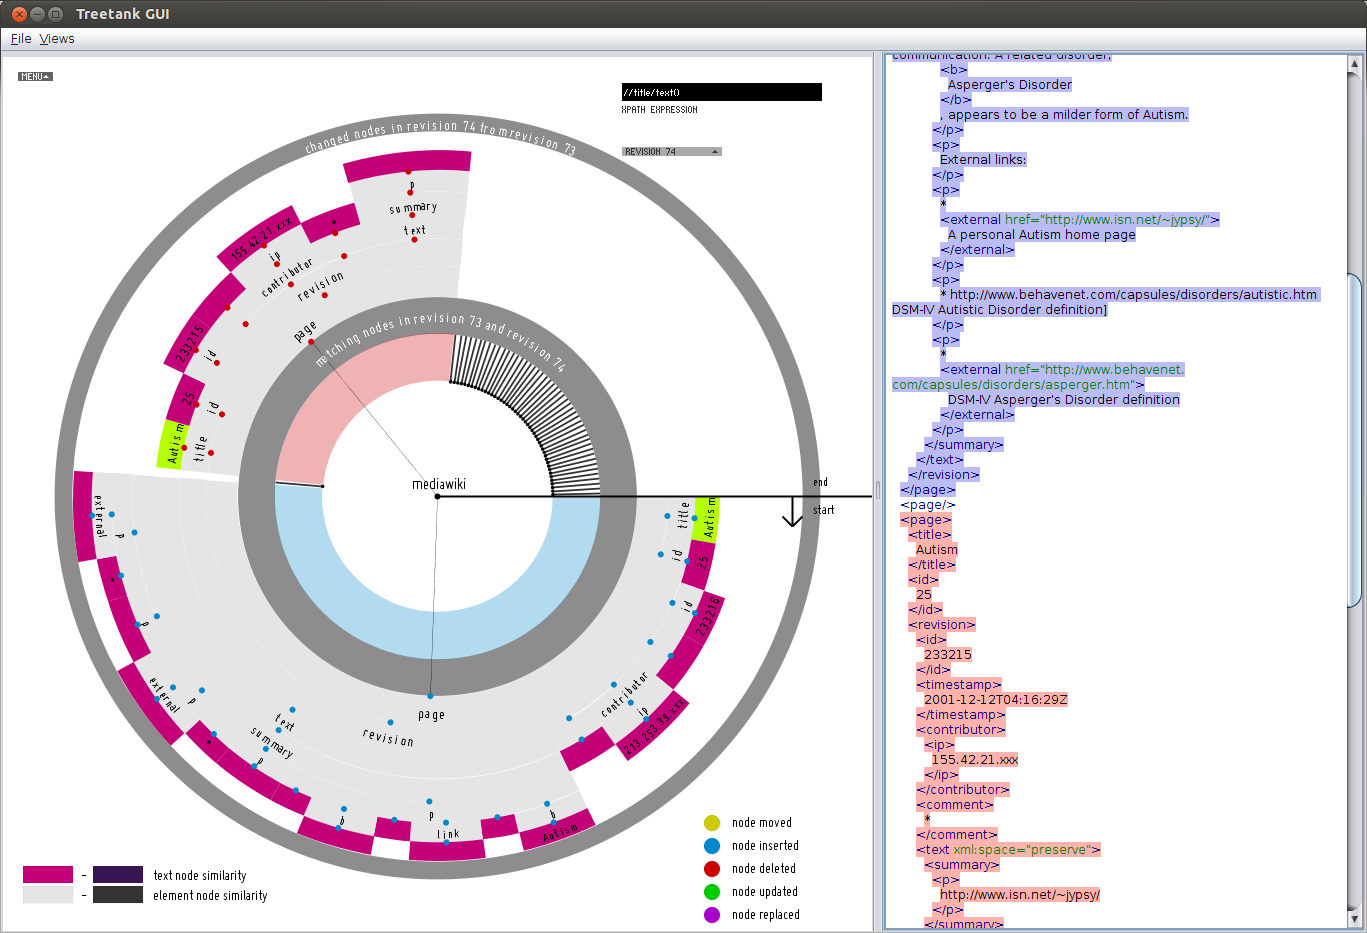
\includegraphics[width=\textwidth]
{figures/wikipedia-rev7374}}
\caption{\label{fig:wikipedia-rev7374} Wikipedia comparsion - depicting differences between revision 73 and 74}
\end{figure}

Fig. \ref{fig:wikipedia-smallmultiple-incremental} finally reveals that between revision 10 and 13 articles are added which is expected. Articles are most probably going to be altered in later revisions once most or all 50 articles have been pre\-pen\-ded. However revision 14 updates an article added in one of the first 10 revisions.

\begin{figure}[tb]
\center{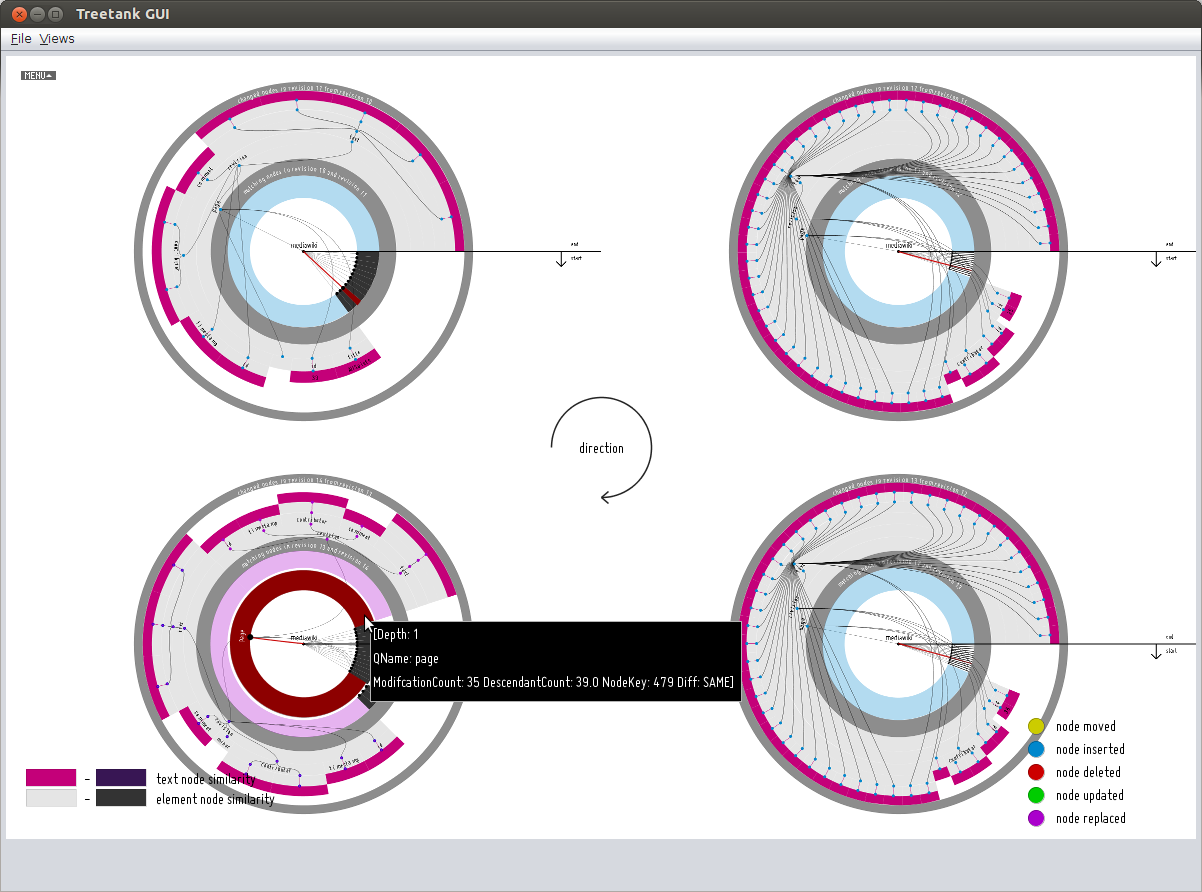
\includegraphics[width=\textwidth]
{figures/wikipedia-incremental-add}}
\caption{\label{fig:wikipedia-smallmultiple-incremental} Wikipedia comparsion - incremental smallmultiple variant depicting changes between revisions 10,11,12,13 and 14 from the upper left to the bottom left in clockwise order.}
\end{figure}

%To further emphasize the changes and to speed up the calculation we can use the pruning-mechanisms described in chapter 4. Using the pruning based on the itemsize results in Fig. \ref{fig:wikivis-pruned-itemsize}. Instead of larger itemsizes for changed nodes potentially uninteresting nodes are pruned away, which are too small and aren't modified between the two compared revisions. Note that these nodes can still be displayed as a user drills down into the tree by selecting a new root-node, whereas all subtree-nodes are scaled according to the new root.

%In order to maximally highligh nodes which are changed between the two revisions Fig. \ref{fig:wikivis-pruned-hash} displays the result of applying the hashbased diff-algorithm. Whenever same hashes are encountered for the two nodes of each revisions the whole subtree is skipped for traversal and as such also in the visualization. As a direct consequence maximal performance as well as itemsize for changed nodes is achieved. Context nodes are preserved, such that all siblings of the root-nodes regardings changes are still visible. As a matter of fact we can still enlarge the items which depict changed-nodes by tuning the variable which denotes, how much modifications are weighted in respect to the number of descedants per node in addition to the current node.

%\begin{figure}[htb]
%\center{\includegraphics[width=\textwidth]
%{figures/wikipedia-50-articles-prunedhash.png}}
%\caption{\label{fig:wikivis-pruned-hash} Wikipedia comparsion pruned by hash-comparsion}
%\end{figure}

%In order to compare sequences of revisions it's also possible to view incremental and differential changes between the loaded base-revision and the other revisions. Fig. \ref{fig:wikipedia-smallmultiples-differential} reveals the initial addition of several article, whereas the articles are not present before. In the last comparsion, the lower left SmallMultiple an article is updated instead of added. In order to zoom into interesting regions and to gain further insights the normal view comparing two revisions can be used which is going to be linked with the SmallMultiplesViews.

%\begin{figure}[htb]
%\center{\includegraphics[width=\textwidth]
%{figures/wikipedia-smallmultiples-differential.png}}
%\caption{\label{fig:wikipedia-smallmultiples-differential} Wikipedia comparsion (differential smallmultiples view)}
%\end{figure}

%Another view (Fig. \ref{fig:wikipedia-smallmultiples-hybrid}) displays the evolution whereas revision 0 is the base revision with just one article added. Afterwards other articles are appended as long as no article has been updated. Articles which haven't change within the two compared revisions are blackened.

%\begin{figure}[htb]
%\center{\includegraphics[width=\textwidth]
%{figures/wikipedia-smallmultiples-hybrid.png}}
%\caption{\label{fig:wikipedia-smallmultiples-hybrid} Wikipedia comparsion (hybrid smallmultiples view)}
%\end{figure}

\subsection{Import of Filesystem-based tree-structure}
Filesystems usually organize data in a tree-structured hierarchy whereas a unique \emph{Path} denotes the location of a file. As a direct consequence it is an optimal use case to demonstrate the feasability of our proposed approach as the tree-structure can not be neglected if we quickly want to detect differences in the folder/file-structure based on snapshots.

Use cases are manyfold, ranging from monitoring software-evolution based on the package/class hierarchy to monitoring if employees stick to organizational policies.

In order to take snapshots of a directory with all subdirectories we study two approachs:

\begin{enumerate}
\item FSML representation based on a python script \cite{FSML}, which is executed several times to obtain snapshots based on an XML-representation which are afterwards imported in Treetank. The differences between the snapshots are calculated based on the FMSE-algorithm described in Chapter 2 and 3.
\item FSML representation based on an initial import of a directory with all its subdirectories. Changes in that directory and all subdirectories are afterwards monitored.
\end{enumerate}

The File System Markup Language\cite{FSML} is an XML-dialect developed by Alexander Holupirek to represent the tree-structure of filesystems by folders and files as well as metadata of certain file-types. 

The first approach is considerably simpler than the import of Wikipedia due to the snapshot-creation which results in different files. Therefore we do not have to reorder whole subtrees according to timestamps in the first place to obtain a subsequent import ordered by time. Instead applying the FMSE-algorithm on the last imported revision and the new XML document is sufficient.

Fig. \ref{fig:fsml-gui} reveals the differences between revision 0 and 4 using the hash-based pruning on manually taken snapshots of the src-folder of our GUI project (slightly outdated) with a Python-script, developed by Alexander Holupirek, too. We are able to detect possible hotspots of development on the package/class-level. It is immediately obvious that a ForkJoin-Quicksort implementation has been deleted recently. Another interesting observation is the recent work on BSplines which have been added to facilitate the Hierarchical Edge Bundling technique described in Chapter \ref{sec::visualizations}. Furthermore we are able to spot recent work on a new \emph{Treemap}-view. The XPath-query \texttt{//element()[@st\_mode="0100664"]} highlights nodes whith the appropriate mode.

\begin{figure}[tb]
\center{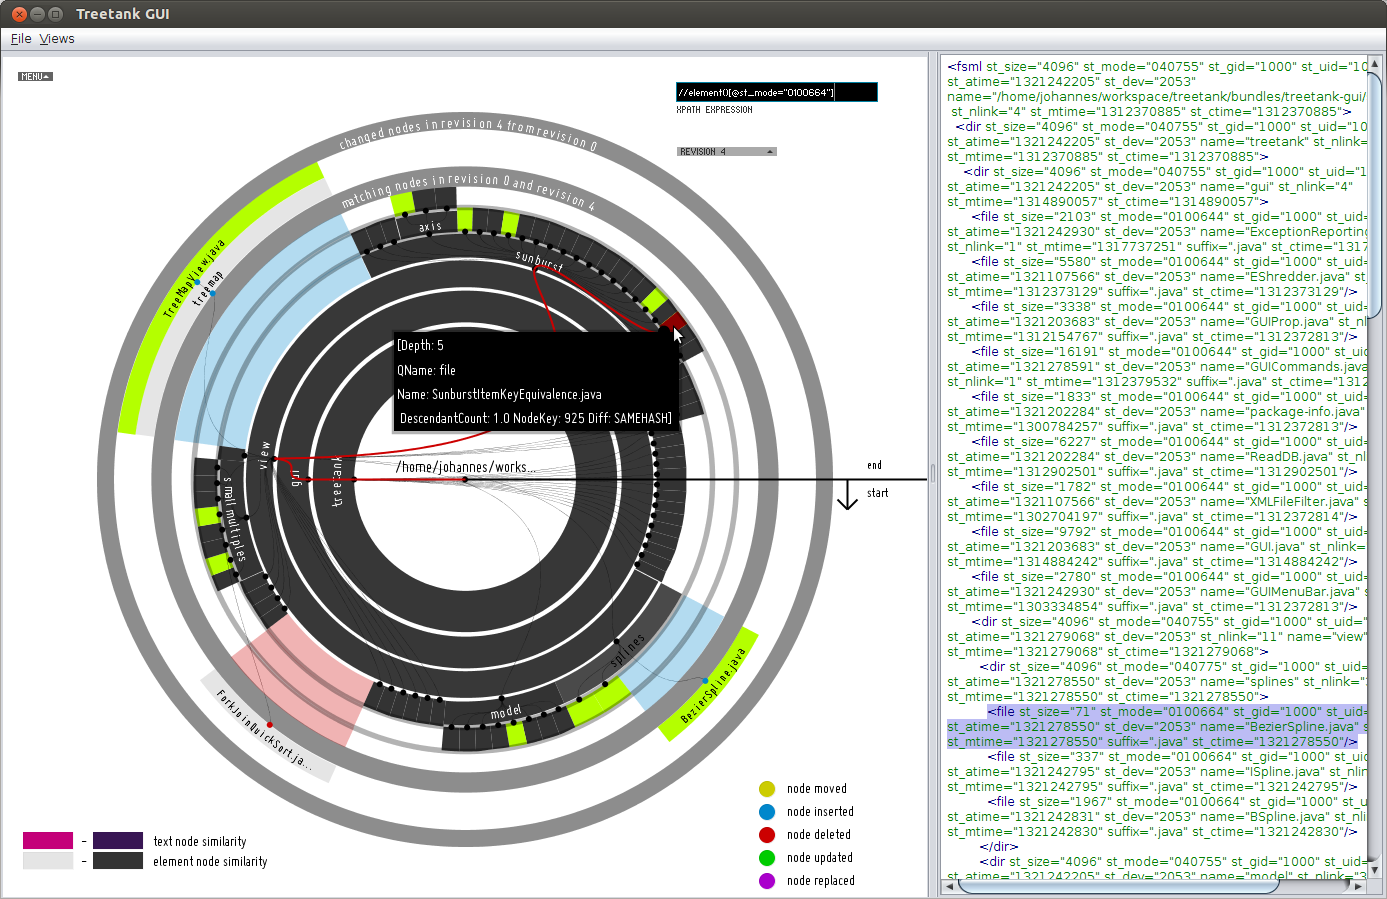
\includegraphics[width=\textwidth]
{figures/fsml-gui}}
\caption{\label{fig:fsml-gui} FSML comparsion on the GUI src-folder}
\end{figure}

The alert reader might think that some of the nodes for instance the subtree of the "sunburst"-subtree which are plotted should not have been processed by the ID-based diff algorithm because we are utilizing the hash-based diffing algorithm, but by close inspection it is revealed that these nodes have different hash values (on mouseover the details are revealed, that is type \texttt{DiffType.SAME} instead of \texttt{DiffType.SAMEHASH}). We currently do not color-encode nodes which have identical hash-values differently to nodes with identical node-IDs but different hash-values. Moreover up until now we have always used the ID-based diffing mode which does not include namespace/attribute comparisons. However, once including checks for namespace/attribute equivalence we are able to detect updates of certain nodes (Fig. \ref{fig:fsml-gui-fulldiff}) due to last access time of a file/directory which is denoted through the \texttt{st\_atime}-attribute. Each time either a namespace- or an attribute-node differs the parent \texttt{ElementNode} is emitted as being updated once the full diff mode is enabled.

\begin{figure}[tb]
\center{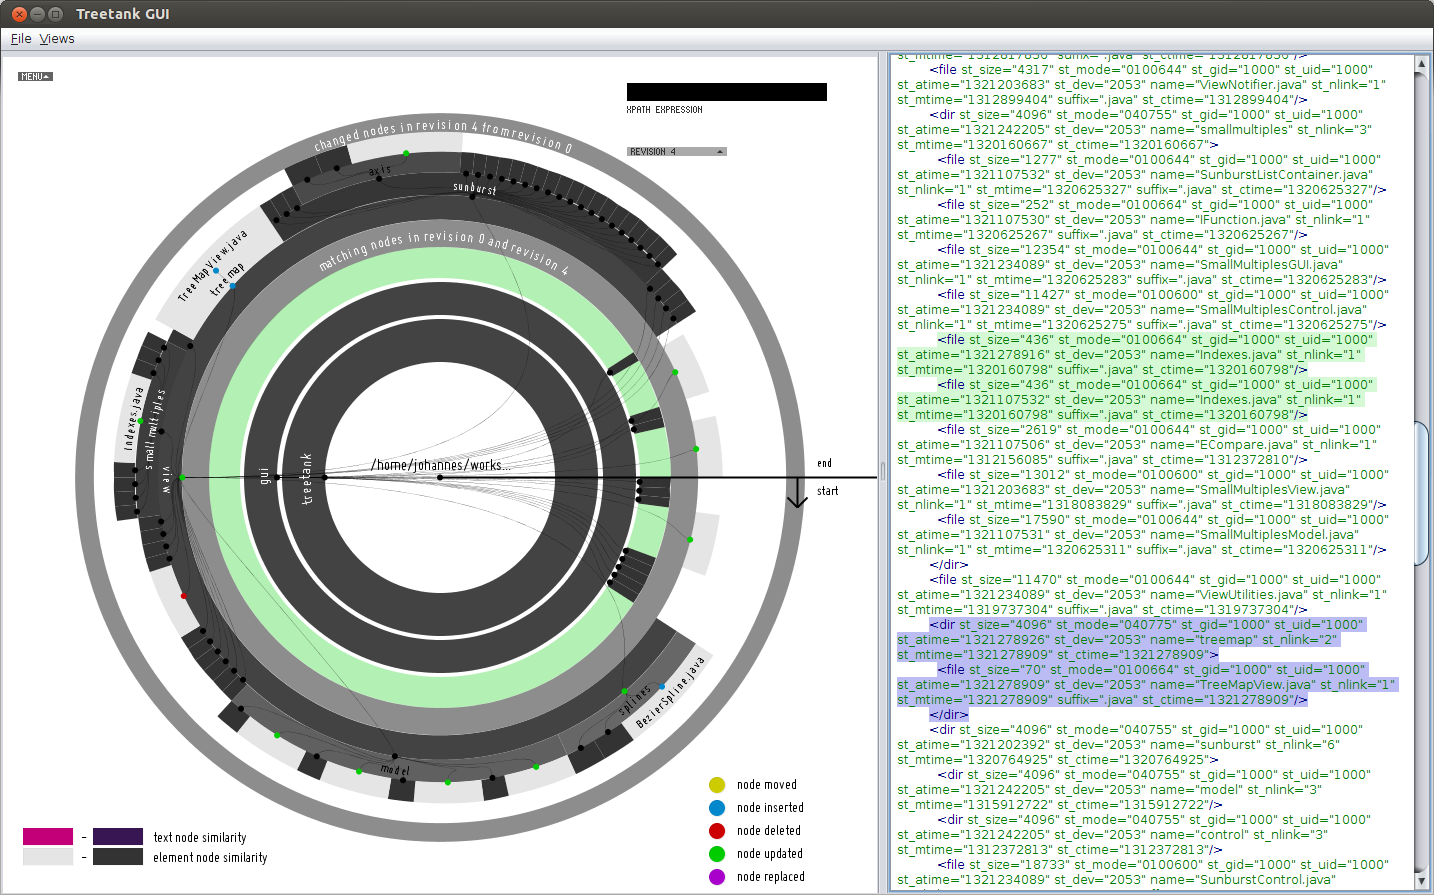
\includegraphics[width=\textwidth]
{figures/gui-fsml-fulldiff}}
\caption{\label{fig:fsml-gui-fulldiff} FSML comparsion on the GUI src-folder using a full diff including namespaces and attributes}
\end{figure}

We conclude, that the preprocessing step of matching nodes in the FMSE-algorithm works reasonably well on FSML-data as no similar \texttt{TextNode}s are included. However we aim to support the extraction of metadata for several kinds of files which might introduce the possibility of mismatches in the future.

In order to avoid any mismatches and therefore executing too many update-operations on nodes which have not changed at all as well as to avoid the costly execution of the FMSE-algorithm in the first place the capabilities of current filesystems to register for modification-events are additionally used. The steps are as follows:

\begin{enumerate}
\item To obtain the hierarchical structure of filesystems the Java7 Filesystem-Walker API is used instead of the Python-Script. A new database is created in Treetank with a standard resource named "fsml" whereas the hierarchical structure is mapped to the resource while traversing a directory. 
\item The new \texttt{WatchService} is used to detect subsequent changes in a watched directory. In order to support watching all subdirectories as well a suitable datastructure as for instance an associative array has to be used in the first place. Java does not permit recursive watching of all subdirectories, as it is not supported by some filesystems.
\end{enumerate}

The \texttt{WatchService} detects the following events:

\begin{itemize}
\item \texttt{ENTRY\_CREATE}: File or directory has been created.
\item \texttt{ENTRY\_DELETE}: File or directory has been deleted.
\item \texttt{ENTRY\_MODIFY}: File has been modified.
\end{itemize}

Therefore moves and renames are not supported out of the box. The path to the directories and files is translated to an XPath query, which locates the appropriate node in the database/resource. In case a new file or directory has been created a new \texttt{ElementNode} is pre\-pen\-ded as a first child of the parent node as filesystem-trees are unordered. In this case the XPath-query translates the parent-path into the appropriate XPath-query, that is it is of the form \\\texttt{/dir[@name='pathComp1Name']/dir|file[@name='pathComp2Name']}. The \\path component usually denotes a directory whereas the last component might be a directory or file in case of an \texttt{ENTRY\_DELETE} event. Deleted directories have to be removed from a WatchService/Path-mapping in an associative array. Furthermore all paths have to be saved in another datastructure to denote if the deleted path pointed to either a file or directory. Thus another associative array is used to save a Path $\Leftrightarrow$ EPath mapping for inserted nodes. EPath is a Java enum to determine the type (file or directory).

\begin{code}[caption=FSML structure]
<fsml>
  <dir name="Desktop">
    <dir name="Lichtenberger">
      <dir name="Bachelor">
        ...
      </dir>
      <dir name="Master">
        <dir name="Thesis">
          <dir name="figures">
            <file name="fsml-incremental.png" suffix=".png"/>
            ...
          </dir>
          <file name="thesis.tex" suffix=".text"/>
          ...
        </dir>
        ...
      </dir>
    </dir>
    ...
  </dir>
</fsml>
\end{code}
\label{lst:fsml}

The FSML-subdialect currently used is very simple. Listing \ref{lst:fsml} provides an example of the simple structure. Directories are mapped to \texttt{dir}-elements, whereas files are mapped to \texttt{file}-elements. Note that the names can not be used without preprocessing to denote the elements, as for instance whitespaces are not permitted in QNames. Thus, either whitespace characters and other not allowed characters are escaped or as in our case saved as attribute-values in \texttt{name=""}-attributes. The labels in the visualizations are optionally based on this special attribute.

While this representation currently does not incorporate most of the strengths FSML usually provides it is easy to add metadata about files and to incorporate text-files. Optionally instances of custom classes are pluggable to provide any type of extensibility. Thus it is possible to provide extractors for certain types of files and to incorporate text-files into the FSML-representation itself, possibly by adding a link to another resource in the fsml-database.

Fig. \ref{fig:fsml-itemsize-pruning} is an example of mapping the author's Desktop-folder to a database in Treetank (move- and replace-detection is disabled). Subsequent revisions are commited every five minutes.

\begin{figure}[tb]
\center{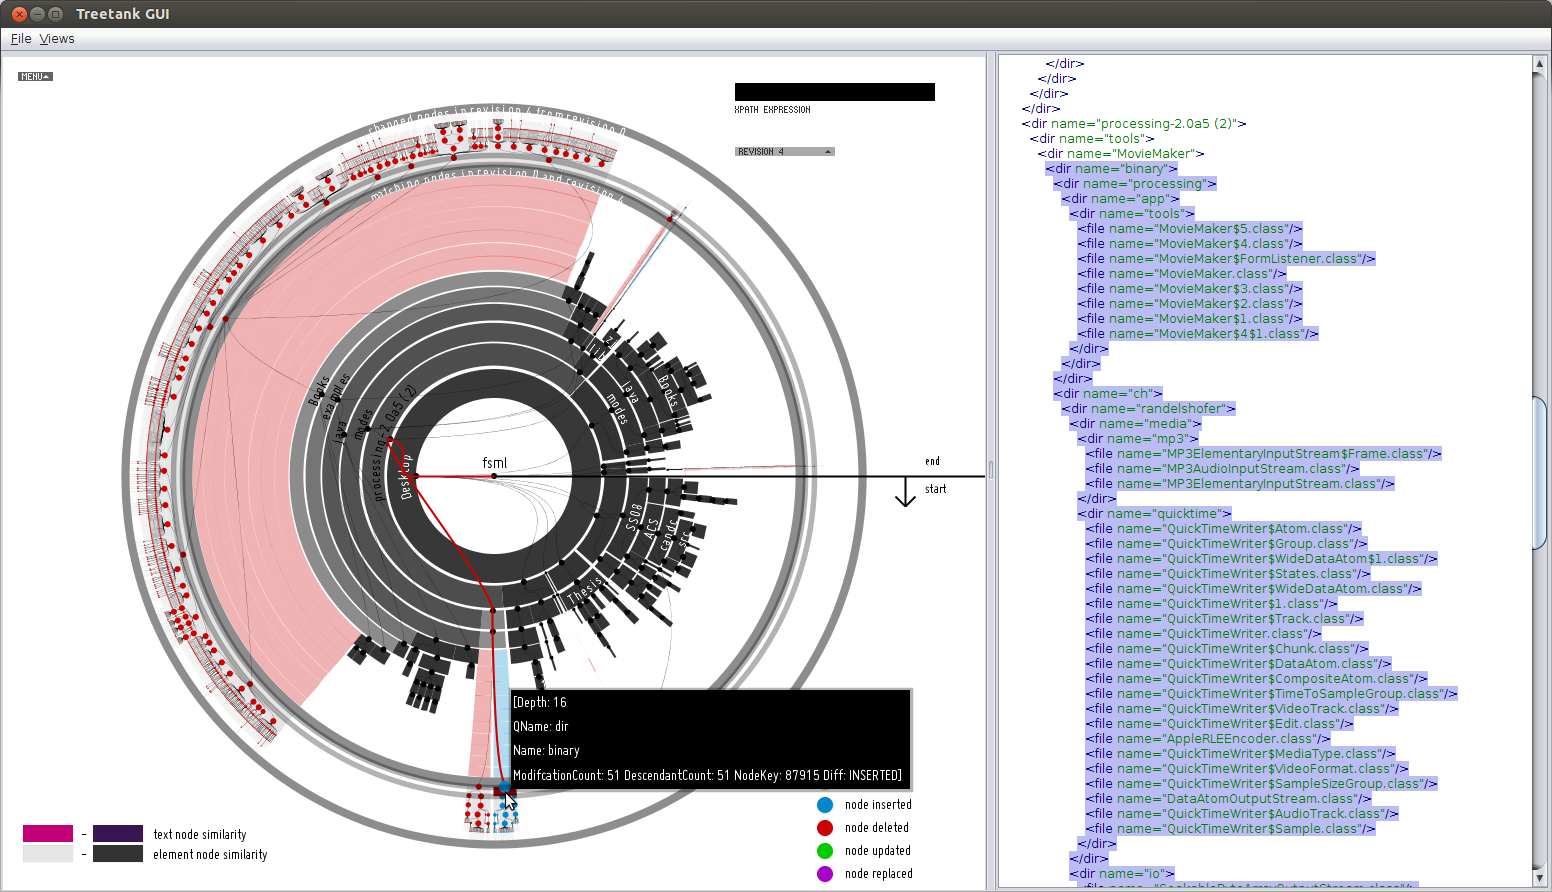
\includegraphics[width=\textwidth]
{figures/fsml-changes-itemsize-pruning.png}}
\caption{\label{fig:fsml-itemsize-pruning} FSML comparsion of "/home/johannes/Desktop"}
\end{figure}

Most files and directories are unchanged. Usually subtrees of changed items (besides the processing-subfolder which has been deleted) are rather small compared to most unchanged nodes. Thus, we study the effect of changing the filtering method. Pruning by same hashes instead of the itemsize is displayed in Fig. \ref{fig:fsml-pruned-by-samehashes}. Sunburst items for the large subtrees of the unchanged nodes are not generated. As a direct consequence items of interest are enlarged and thus much better visible. %Two subdirectories matching the simple XPath-query \texttt{//dir[@name='wiki-sorted']} are highlighted. It is immediately obvious that a subtree rooted at the directory named "wiki-sorted" has been deleted and another one has been inserted. The equal subtree-size suggests that the subtree has been moved. On close inspection, for instance using the subtrees rooted at "wiki-sorted" we see that the subtrees are isomorph (Fig. \ref{fig:desktop-screenshot-compare}). This might be due to the directory traversal which seems to be non-deterministic. We can suggest that the directory therefore has been moved. However in future work we aim to detect moves in the first place and therefore also use the appropriate visualization through splines explained in chapter 3. To compare the two subtrees we used two Treetank-GUI instances on the same database/resource. This is possible due to Treetank permitting multiple read-transactions.  

\begin{figure}[tb]
\center{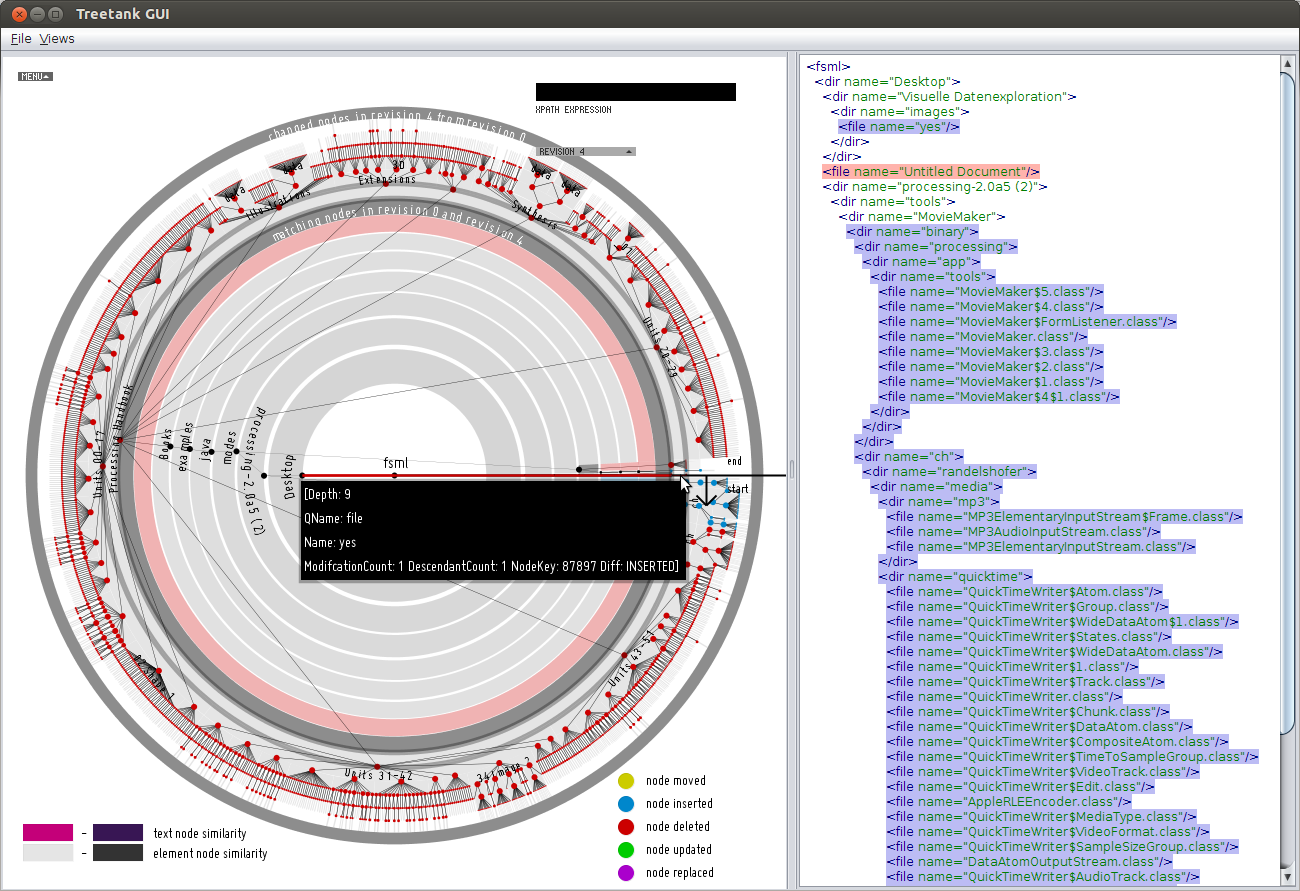
\includegraphics[width=\textwidth]
{figures/fsml-pruned-by-hashes}}
\caption{\label{fig:fsml-pruned-by-samehashes} FSML comparsion of "/home/johannes/Desktop" pruned by same hashes}
\end{figure}

%\begin{figure}[tb]
%\center{\includegraphics[width=\textwidth]
%{figures/desktop-screenshot-compare.png}}
%\caption{\label{fig:desktop-screenshot-compare} FSML comparsion of wiki-sorted subtrees}
%\end{figure}

%To reduce the number of \emph{SunburstItem}s and the runtime of creating the items and the offscreen buffer the tree can be pruned by itemsize, just like in the case of the wikipedia-import. Items which are too thin and thus do not add any value to the visualization are pruned. The default modification-weight is used, which is not enough to adjust and enhance the sizes of changed subtrees. Furthermore this type of pruning doesn't impose any positive effect on the subtree-size of changes. Therefore we use the pruning by hash-values (Fig. \ref{fig:desktop-screenshot-pruned-hash}), which skips any unchanged subtrees. The number of created items is reduced drastically without causing any negativ effect. The context is still visible. Furthermore the items are big enough to be readable on the highest level without zooming into subtrees by selecting a new subtree-root node.

%\begin{figure}[htb]
%\center{\includegraphics[width=\textwidth]
%{figures/desktop-screenshot-pruned-hash.png}}
%\caption{\label{fig:desktop-screenshot-pruned-hash} FSML comparsion of "/home/johannes/Desktop" pruned by same hashes}
%\end{figure}

A sequence of comparisons between several revisions is viewable with the incremental small multiple display variant (Fig. \ref{fig:fsml-smallmultiples-incremental}). We used the hash-based pruning without generating items for nodes with identical hash-values, to keep the number of items to a minimum. By hovering the items and comparing the values as well as subtree sizes we are able to determine a directory-rename between revision 2 and 3 in the bottom right view. A \texttt{rename}-operation however is not supported by the Java \texttt{WatchService} such that usually, depending on the filesystem a delete- and an insert-event in either order is received.

In general we are able to answer questions such as 

\begin{itemize}
\item Auditing: Which files are updated/inserted/deleted or not during a sequence of snapshots?
\item Does an employee adhere to company instructions regarding installed software? (by file-extensions or analysing the binaries and storing an additional attribute with "true" or "false" values)
\end{itemize}

\begin{figure}[tb]
\center{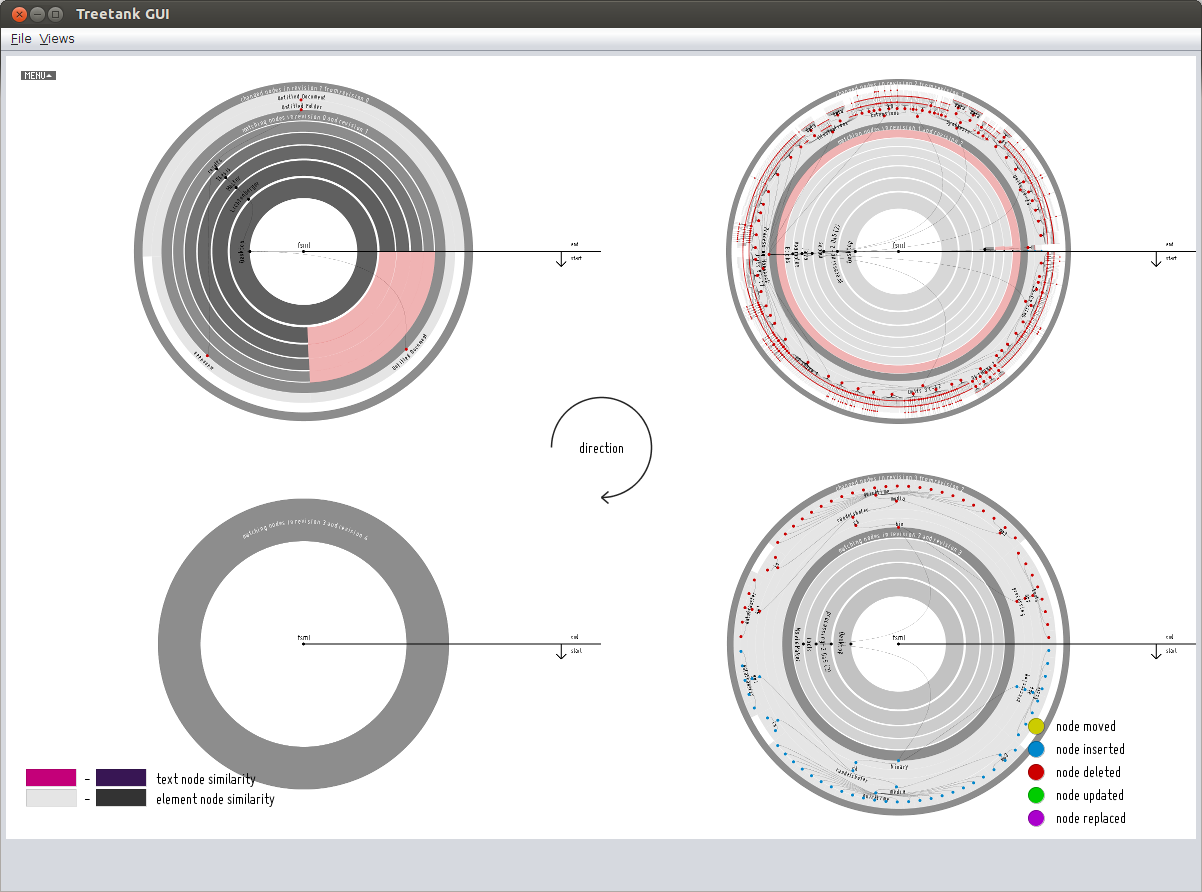
\includegraphics[width=\textwidth]
{figures/fsml-incremental-pruned-by-samehashes.png}}
\caption{\label{fig:fsml-smallmultiples-incremental} FSML comparsion of "/home/johannes/Desktop" (small multiple displays -- incremental view)}
\end{figure}

\subsection{Summary}
This chapter introduced a few use cases for comparing tree-structures. Depending on the activated views different characteristics are revealed. 

The smallmultiple differential-variant should be used to compare similar, different tree structures. Choosing the incremental variant reveals changes in temporal evolving trees. In case the tree is rather small (for instance less than 5000 nodes) it is arguable that the views can be used without filtering. However, once more items have to be created it is necessary to choose one of the filtering techniques to keep the numer of items small and to prune nodes/subtrees of no interest. Hovering through linking and brushing facilitates keeping track of changed nodes. When one of the pruning techniques is enabled, inserted nodes might not be visible in upcoming comparisons. However, this indicates that the items have not been changed within later revisions. 

The standard \emph{SunburstView} reveals all kinds of differences and furthermore allows two zooming operations. The zooming/panning which transforms the viewing-coordinates through affine transformations may be used if the number of items is small and therefore animations are possible whereas a left-mouseclick on an item transforms the item into a new root-node. As already explained in Chapter \ref{sec::visualizations} this involves either a transformation based on node-copies and adjusting angles or the full pipline has to be passed in case of the itemsize-pruning.

We have merely scratched the surface of the possibilities of our current approach. The small multiple displays will greatly benefit from a temporal XPath-extension. Some proposed axis as \texttt{next::}, \texttt{previous::}, \texttt{future::}, \texttt{past::}, \texttt{revision::} already have been implemented but have to be incorporated in an XPath/XQuery-engine. Simple queries as for instance \\\texttt{//dir[@name='wiki-sorted']/future::node()} will reveal nodes with the attribute \texttt{name='wiki-sorted'} in all future revisions. The start-context will be based on the currently opened base-revision. 
